\subsection{Evaluation der Komponenten} \label{kap:Evaluation_der_Komponenten}
\textit{(pro)} Nachdem der konzeptionelle Aufbau der Maschine in den vorangehenden Unterkapiteln ausführlich ausgearbeitet wurde, werden in diesem Unterkapitel die für die Funktion der Maschine benötigten Einkaufkomponenten evaluiert. Dabei werden die zu beschaffenen Komponenten systematisch nach den drei Maschinenteilen Setzeinheit, Vereinzelung und Verstellmechanik behandelt. Zu jeder Teilfunktion werden zuerst die mechanischen und anschliessend die elektronischen Komponenten besprochen.

\subsubsection{Setzeinheit} \label{subsec:Translation}
\textbf{mechanische Komponenten}\\
\textit{(ygu)} Für die Realisierung der translatorischen Bewegung der Setzeinheit bieten sich verschiedene Technologien an. In der Automatisation werden folgende Realisierungen verbreitet eingesetzt:
	\begin{itemize}
	\item \textbf{Spindelantriebe:}
	Ein Motor treibt eine gelagerte Spindel an. Durch eine Bewegungsschraube wird die Rotation in eine Translation gewandelt. Spindeln sind preiswert, bieten eine hohe Gestaltungsfreiheit und sind vielfältig einsetzbar. Für Anwendungen mit hohen Geschwindigkeiten kommen Steilgewindespindeln zum Einsatz. Nachteilig ist der höhere Entwicklungsaufwand.
	\item \textbf{Elektrozylinder:}
	Elektrozylinder werden als fertige Komponenten eingekauft und sind in ihrer Funktionsweise mit jene der Spindeln identisch. Im Innern befindet sich auch eine Spindel, welche über einen Riemenantrieb oder Getriebe vom Motor angetrieben wird. Diese Fertigteile erreichen Geschwindigkeiten bis 600 mm/s und 15kN Axialkraft. Verglichen mit Spindeln sind Elektrozylinder in der Anschaffung wesentlich teurer.
	
	\item \textbf{Pneumatik:}
	Auch die Pneumatik bietet Lösungen für die Anwendung. Dabei wird Druckenergie in kinetische Energie umgewandelt. Ein Pneumatikzylinder kann die geforderte Geschwindigkeit und Kraft für diese Anwendung aufbringen. Die einfache Implementation und Ansteuerung sind klare Vorteile. Jedoch sind Pneumatikkomponenten teuer und benötigen einen Druckluftkompressor.
	\end{itemize}

Durch den Setzprozess und die Geometrie der Töpfe sind folgende Anforderungen gegeben:
\begin{table}[H]
\begin{tabular}{|l|l|l|}
	\hline 
	Parameter & Wert & Kommentar \\ 
	\hline 
	Einschaltdauer ED & 50\% & gegeben durch Topfmaschine \\ 
	\hline 
	Mittlere Axialkraft F\textsubscript{axavg} & 20N & Aus Funktionnachweis (vgl. Kap. \ref{nemacaps_setzen}) \\ 
	\hline 
	Drehzahl für Spindel n\textsubscript{s}& 3000 U/min & überschlägige Annahme \\ 
	\hline 
	Beschleunigungsdrehmoment M\textsubscript{a}& 0.36 Nm & überschlägige Annahme \\ 
	\hline 
	mittlere Geschwindigkeit v\textsubscript{avg}& 500mm/s & überschlägig gemäss Gleichung 1\\ 
	\hline 
\end{tabular} 
\caption{Anforderungen an den Setzprozess}
\label{tab:annahmen_setzeinheit}
\end{table}
\begin{equation}
v_{avg}=\frac{2*s_{max}}{T_{min}-T_{t}}=\frac{2*100mm}{0.5s-0.1s}=500mm/s
\end{equation}
\newline
Für die Evaluation der Translation wurden alle drei Technologien unter Berücksichtigung der genannten Anforderungen in Betracht gezogen. Obwohl die Pneumatik die einfachste Umsetzung bietet, kommt diese nicht in Frage. Diese Entscheidung wird mit den hohen Kosten un dem Fehlen von Pneumatikanschlüssen bei der Topfmaschine begründet.
\newline
Da zwischen dem Spindelantrieb und dem Elektrozylinder keinen funktionellen Unterschied feststellbar ist, wurde die Wahl aufgrund der Verfügbarkeit und Preis beurteilt. Im Gespräch (29.3.17) mit dem betreuenden Dozenten wurde Igus als kompetenter Hersteller von Spindeln genannt. Für Elektrozylinder wurden verschiedene Distributoren (Tecalto AG, Bachofen AG, Parkem AG, Phoenix Mecano Komponenten AG) angefragt. Nur Parkem AG konnte ein Produkt zur Offerte anbieten. Somit ergibt sich folgende Gegenüberstellung:
\begin{table}[H]
\begin{tabular}{|c|c|c|}
	\hline 
	Produkt & Igus Ds14x30 & Parkem ETH032  \\ 
	\hline 
	Typ & Spindel & Elektrozylinder \\ 
	\hline 
	Preis [CHF] & <100  & 1700    \\ 
	\hline 
	Lieferfrist [Wochen] &1 - 2  &6 \\ 
	\hline 
\end{tabular}
	\vspace{0.2cm}
	\caption{Vergleich Spindel versus Elektrozylinder}
	\label{tab:spindelauslegung}
\end{table}
Unschwer erkennt man, dass der Preis eines Elektrozylinders um ein Vielfaches höher ist als eine Spindel. Relativieren kann man dieses Argument, wenn man bedenkt, dass für die Spindel ein Motor und die Lagerung beschafft werden muss. Entscheidend ist jedoch das zeitliche Argument. Unter Berücksichtigung des Projektplans wird rasch ersichtlich, dass eine Lieferfrist von 6 Wochen nicht mit der Umsetzung vereinbar ist. Somit wird die Translation mit einer Igus Dryspin Steilgewindespindel realisiert.\\

\textbf{Antriebskomponenten}\\
\textit{(pro)} Der Spindelantrieb stellt die grössten Anforderungen an einen leistungsfähigen Motor inklusive Ansteuerung und Speisung innerhalb dieses Projektes. Naheliegend ist deshalb auch, dass es sich hierbei um die teuersten Komponenten des Elektronik Konzepts handelt. Die Anforderungen an den Spindelantrieb wurden gemäss Tabelle \ref{tab:spindelauslegung} in erster Annahme wie folgt festgelegt: 

\begin{itemize}
	\item Drehzahl = 3090 U/min
	\item Drehmoment = 0.36Nm	
\end{itemize}

%Die mittlere Drehzahl ist dabei nicht als maximale Drehzahl des Motors auszulegen. Sie definiert die Drehzahl welche der Antrieb erreichen muss um den geforderten Vorschub der Spindel von 0.6m/s zu erreichen. Dabei sind die Beschleunigungs- sowie Verzögerungsphasen der Bewegung nicht berücksichtigt. Werden diese unter der Annahme einer linearen Beschleunigung sowie Verzögerung der Spindel über den gesamten Bewegungsablauf miteinbezogen, ergibt sich die maximale Antriebsdrehzahl aus der doppelten mittlere Drehzahl. 

%\textbf{Das erforderliche Drehmoment beschreibt die Übersetzung von geforderter Axialkraft = 32N in das aufzubringende Drehmoment an der Spindelwelle. Die Beschleunigung der Massenträgheit der Setzeinheit muss als zusätzliches Drehmoment addiert werden. Annahme!?!?} Die Berechnungen sowie eine Abbildung der beschriebenen Bewegungsphasen sind in Kapitel \ref{sec:Umsetzung_Spindel} nachzulesen. Die Anforderungen an den Spindelantrieb betragen nach Berücksichtigung dieser Punkte: Merf = 0.36Nm / Uerf = 3090 U/min.

Die hohen Anforderung an die Dynamik des Antriebs stellen nebst den Leistungsdaten ein zusätzliches Evaluationskriterium dar. Die Wahl der Antriebstechnologie fand zwischen den drei am weitesten verbreiteten Antriebsmöglichkeiten für Automatisierungsprozesse statt: Schrittmotoren, DC Motoren und BLDC Motoren. In Abbildung \ref{fig:Motorentypen} sind generelle Vor- und Nachteile dieser Antriebssysteme kurz zusammengefasst. Die in der Abbildung beschriebenen Punkte sind allgemein und nicht auf die spezifische Anwendung bezogen.\\
Eine Lösung mit Schrittmotor wäre aufgrund der einfachen Ansteuerung, bei den geforderten Leistungsdaten die günstigste Variante. Da Schrittmotoren keine Feedback Sensorik zur Regelung der Drehzahl benötigen. Entscheidender Nachteil von Schrittmotoren ist deren schlechteres dynamisches Verhalten. So nimmt das Drehmoment bei steigender Drehzahl ab. Weiter kann ein Schrittmotor, durch das Risiko eines Schrittverlustes, bei gleichem Nennmoment nicht so stark beschleunigt werden wie beispielsweise ein DC oder BLDC Motor. Schrittmotoren müssen bezogen auf die Leistungsdaten demnach um ein vielfaches höher ausgelegt werden als sie effektiv im normalen Betrieb benötigen. Ein weiterer negativer Punkt von Schrittmotoren ist ihre schlechte Laufruhe. Diese kann durch die Verwendung von Microsteps verbessert werden, führt dann jedoch wieder zu einem Drehmomentverlust. 

\begin{figure}[H]
	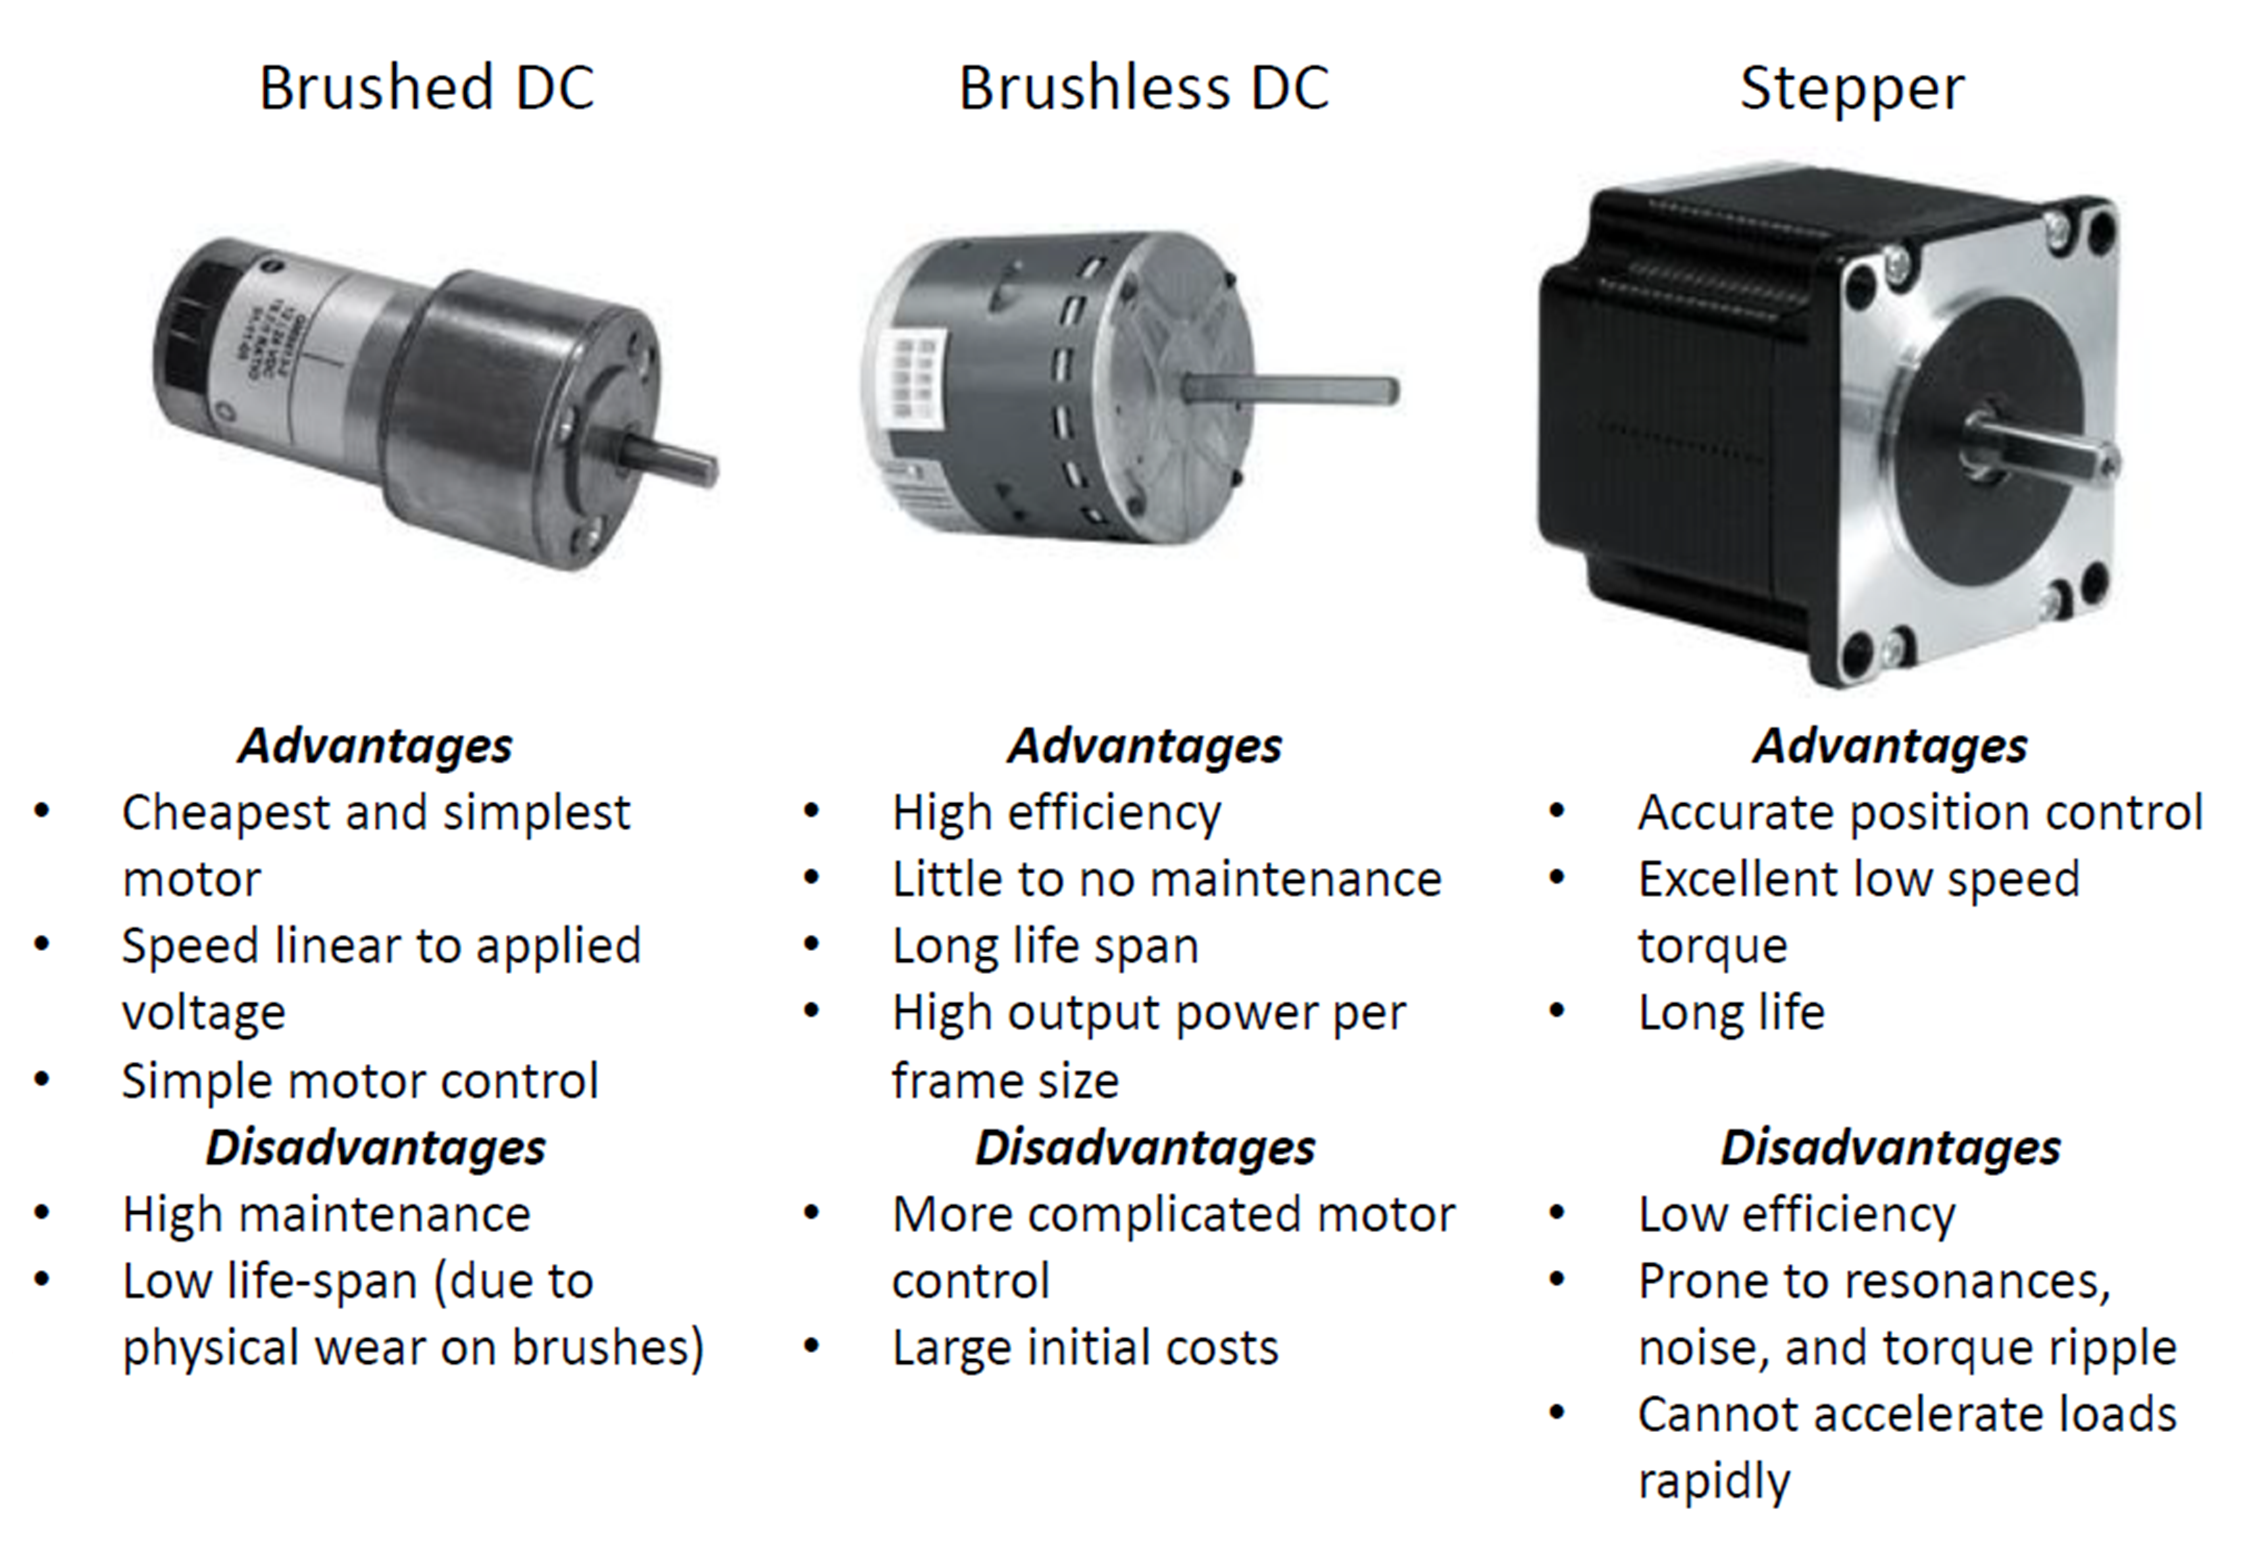
\includegraphics[scale=0.55]{Illustrationen/5-Konzept/Motorentypen.png}
	\caption{Übersicht Motorentypen \protect\cite{Motorentypen}}
	\label{fig:Motorentypen}
\end{figure}

Eine weitaus bessere Lösung bietet somit ein DC oder BLDC Motor. Die beiden Motoren unterscheiden sich im wesentlichen in der Lebensdauer. Da bürstenbehaftete DC Motoren aufgrund der Schleifkontakte zum Rotor besonders bei hoch dynamischen Anwendungen eine sehr begrenzte Lebensdauer haben, wird für diese Anwendung ein BLDC Motor verwendet. Die höheren Kosten für die Steuerelektronik werden dafür in Kauf genommen.\\
Der Markt an Elektromotoren ist gross, dementsprechend schwierig gestaltet sich die Suche für einen passenden Antrieb. Da für diese Anwendung eine Komplettlösung bestehend aus Motor und Steuerelektronik mit Positionierungsreglung gesucht ist, wurde bei namhaften Herstellern solcher Systemkomponenten recherchiert. Folgende Hersteller wurden konsultiert: Maxon Motor, Trinamic und Nanotec. Maxon Motor bietet die grösste Auswahl an Motoren inkl. Zubehör. Diese sind jedoch um den Faktor zwei bis drei Mal so teuer wie die Lösungen von Trinamic und Nanotec. Nanotec bietet in der gesuchten Leistungsgrössenordnung nur Lösungen im Zusammenhang mit CAN Open oder Feldbus Steuerungen an. Die Wahl fiel somit auf die Lösung von Trinamic mit dem Motorentyp QBL5704-116-04-042 und der entsprechenden Steuerung TMCM-1630-2C. In Abbildung \ref{fig:Trinamic}, sowie in Tabelle \ref{tab:Trinamic} sind die Komponenten illustriert.


\begin{figure}[H]
	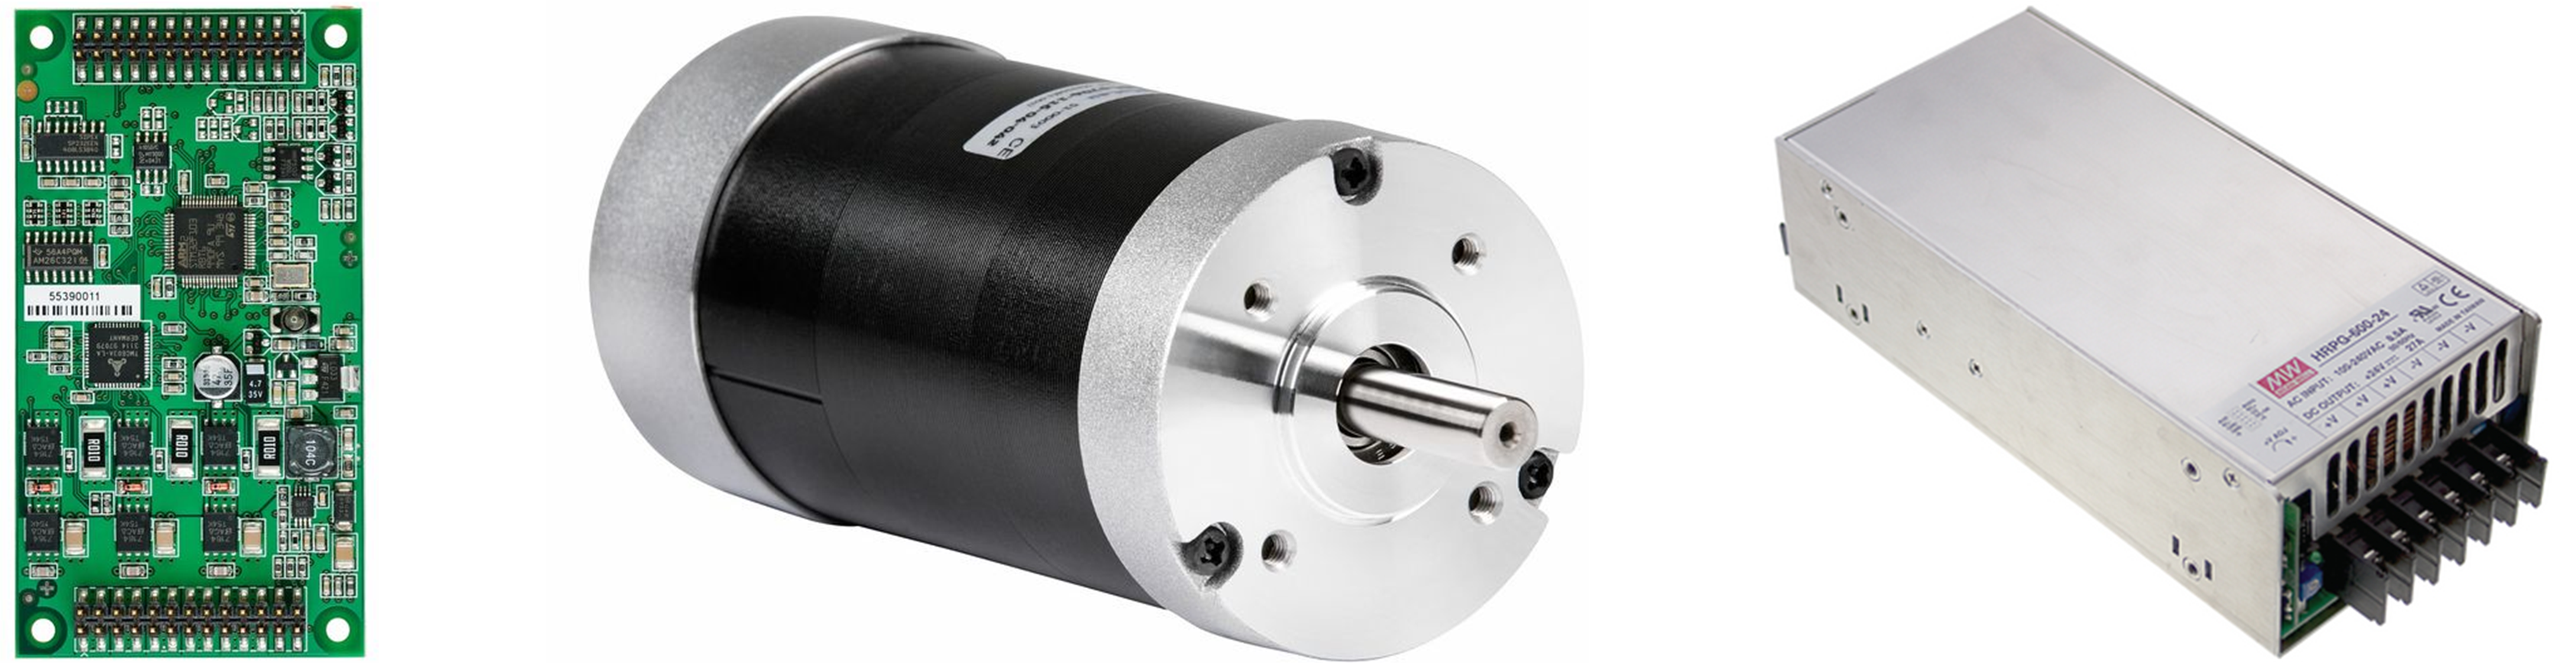
\includegraphics[width=1\textwidth]{Illustrationen/5-Konzept/Trinamic.png}
	\caption{Antriebskomponenten Setzeinheit \protect\cite{Trinamic} \protect\cite{36V_Netzteil}}
	\label{fig:Trinamic}
\end{figure}

\begin{table}[H]
	\centering
	\caption{Antriebskomponenten Setzeinheit \protect\cite{Trinamic} \protect\cite{36V_Netzteil}}
	\begin{tabular}{|l|c|c|c|}
		\hline 
		 & \textbf{Steuerung} & \textbf{Motor} & \textbf{Netzteil} \\
		\hline
		Bezeichnung & TMCM-1630-2C & QBL5704-116-04-042 & HRP-600-36 \\
		\hline
		Nennspannung [V] & 12… 55 & 36    & 36 \\
		\hline
		Nennstrom [A] & -     & 6.67  & 17.5 \\
		\hline
		max. Phasenstrom [A] & 10    & 20.5  & - \\
		\hline
		Nenndrehmoment [Nm] & -     & 0.42  & - \\
		\hline
		max. Drehmoment [Nm] & -     & 1.3   & - \\
		\hline
		Nenndrehzahl [1/min] & < 100'000 & 4000  & - \\
		\hline
		Preis [CHF] & 181.20 & 189.30 & 156.80 \\
		\hline
	\end{tabular}
	\label{tab:Trinamic}
\end{table}


Für die Spannungsversorgung kommt das 36V Netzteil von Mean Well mit der Typenbezeichnung HRP-600-36 zum Einsatz. In Tabelle \ref{tab:Trinamic} sind die wichtigsten Eckdaten des Netzteils aufgelistet. Das Netzteil kann über das Digital Input Signal DC OK vom FRDM-Board ein und ausgeschaltet werden.


\subsubsection{Vereinzelung und Verstellmechanik}
Die beiden Maschinenteile Vereinzelung und Verstellmechanik wurden in einem Kapitel zusammengefasst, weil sie ähnliche Anforderungen an den Antrieb stellen. Gemäss Abbildung \ref{fig:Motorentypen} über die verschiedenen Motorentypen kommen auch hier wieder dieselben Kriterien zur Auswahl des geeigneten Motorentypes zum Einsatz. Das erforderliche Drehmoment für die beiden Funktionen zu schätzen ist sehr schwierig, da lediglich Reibungsdrehmomente als Last vorliegen. Für beide Maschinenteile wurden deshalb DC-Getriebemotoren mit Encoder als die beste Lösung evaluiert. Sie entwickeln bei minimalen Kosten durch die Getriebeübersetzung ein hohes Drehmoment welches eine sichere Funktion garantiert. Die minimale Drehzahl für die Vereinzelung ergibt sich aus der Anzahl Töpfe pro Minute, der Anzahl Lochreihen pro Umdrehung der Lochmaske und einen Sicherheitsfaktor S für die Zeit, in welcher die Lochmaske still stehen soll um die NemaCaps fallen zu lassen:

\begin{equation}
	n = \frac{ N_{Toepfe pro Minute}}{ N_{Lochreihen}} \cdot S  = \frac{60\frac{1}{min}}{6} \cdot 3 = 30\frac{1}{min}
\end{equation}

Die Drehzahl für die Verstellmechanik ist für das Timing des Setzprozesses nicht relevant. Sie kann deshalb fast beliebig klein sein. Wichtig ist hierbei, aufgrund der kleinen Winkeldistanz von 60° welche die Verstellmechanik von Anschlag zu Anschlag besitzt, eine hohe Auflösung des Encoders. Diese wird durch eine möglichst hohe Getriebeübersetzung erreicht. Der Elektronikkomponenten Hersteller Pololu bietet kostengünstige DC-Getriebemotoren mit Encoder in diversen Getriebeausführungen an. Für die Vereinzelung sowie die Verstellmechanik werden Motoren vom Typ 25D mm mit Encoder verwendet. In Tabelle \ref{tab:12V_Antriebskomponenten} sind die beiden Motoren beschrieben, in Abbildung \ref{fig:12V_Antriebskomponenten} ist der Motorentyp 25D mm abgebildet.

\begin{figure}[H]
	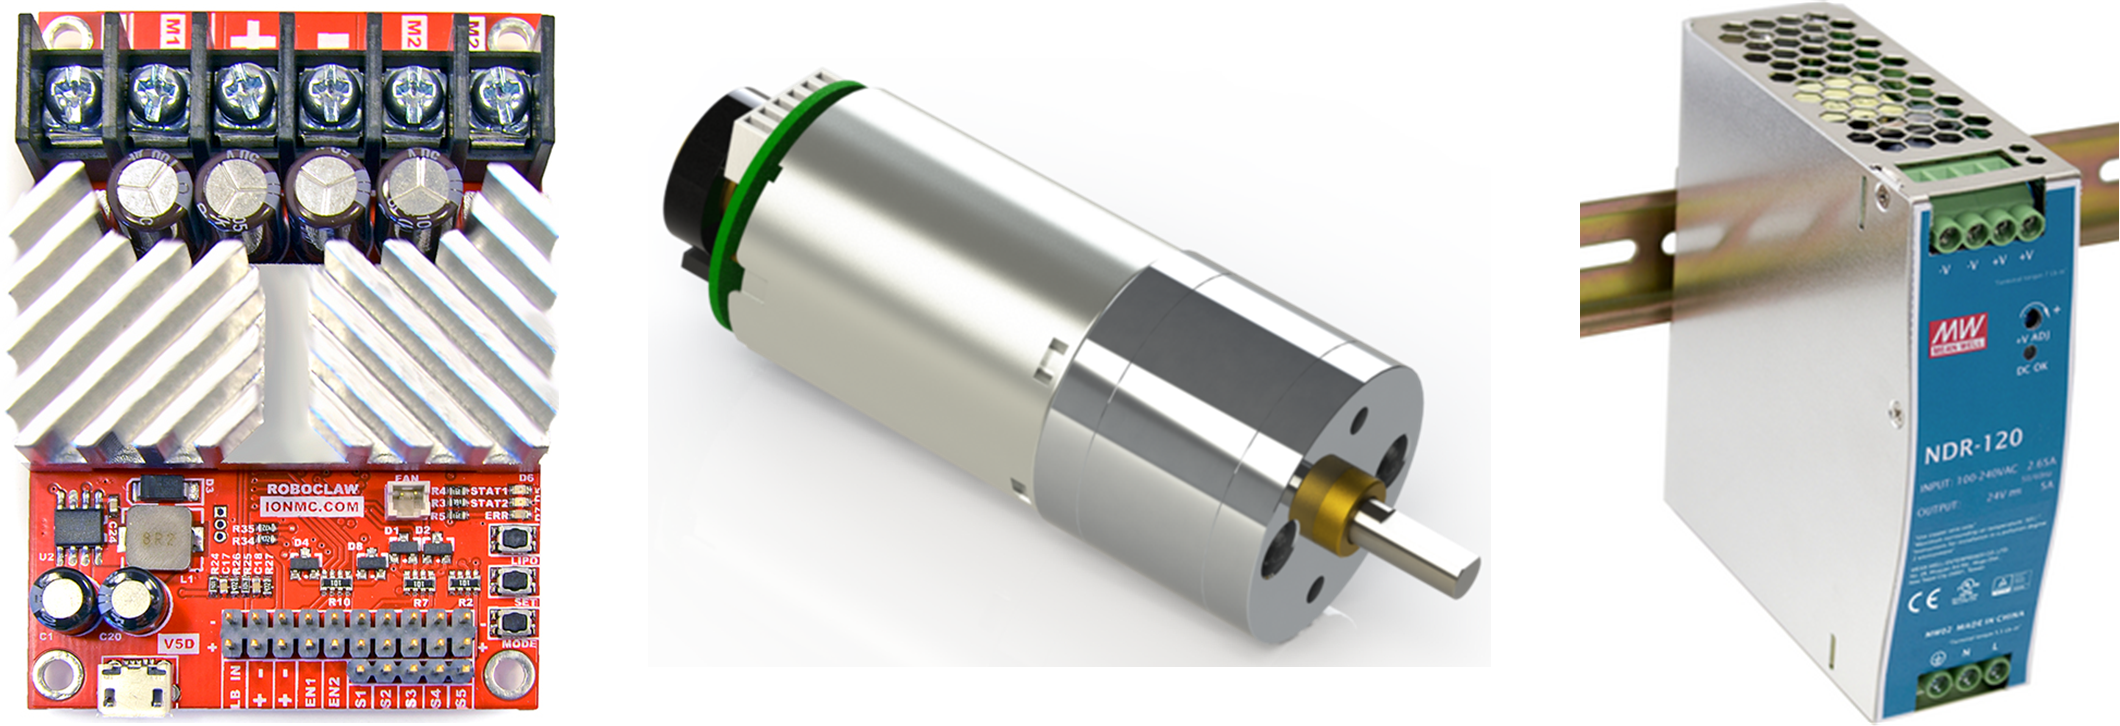
\includegraphics[width=1\textwidth]{Illustrationen/5-Konzept/12V_Antriebskomponenten.png}
	\caption{Antriebskomponenten 12V \protect\cite{ION_Motion} \protect\cite{Pololu_Motors} \protect\cite{12V_Netzteil}}
	\label{fig:12V_Antriebskomponenten}
\end{figure}

\begin{table}[H]
	\footnotesize
	\centering
	\caption{Antriebskomponenten 12V \protect\cite{ION_Motion} \protect\cite{Pololu_Motors} \protect\cite{12V_Netzteil}}
	\begin{tabular}{|l|c|c|c|c|}
		\hline
		& \textbf{Steuerung} & \textbf{Motor Vereinz.} & \textbf{Motor Verstellm.} & \textbf{Netzteil} \\
		\hline
		Bezeichnung & RoboClaw 2x15A & 99:1, 25Dx54L mm & 378:1, 25Dx58L mm & NDR-120-12 \\
		\hline
		Nennspannung [V] & 6… 34 & 12    & 12    & 12 \\
		\hline
		Nennstrom [A] & 15    & -     & -     & 10 \\
		\hline
		max. Phasenstrom [A] & 30    & 5.6   & 1.1   & - \\
		\hline
		Anlauf Moment [Nm] & -     & 2.1   & 2.3   & - \\
		\hline
		Nenndrehzahl [1/min] & -     & 100   & 14    & - \\
		\hline
		Preis [CHF] & 89.95 & 36.95 & 34.95 & 40.95 \\
		\hline
	\end{tabular}
	\label{tab:12V_Antriebskomponenten}
\end{table}

Die beiden Motoren werden über den RoboClaw 2x15A Motorencontroller angesteuert. Dieser Motorentreiber besitzt 2 Kanäle mit jeweils 15A Nennstrom. Es wurde explizit die Variante mit 15A Phasenstrom evaluiert, weil diese über eine interne 5V / 3A Spannungsquelle verfügt, welche auf dem Mainboard das Servo Interface speist. Der Controller verfügt über eine UART Schnittstelle zur Kommunikation mit dem FRDM-Board. Ausserdem ist er mit einer Micro-USB Buchse bestückt. Über das USB Interface kann der Controller mit dem Programm $"$ION Studio Setup App$"$ von ION Motion über den Computer konfiguriert und angesteuert werden. Der Controller ist in der Lage die Motoren, unter Verwendung der Encoder, in einer Positionsregelung zu betreiben.\\
Das 12V Netzteil von Mean Well ist für die Spannungsversorgung der Motoren sowie der Elektronik Komponenten des Mainboards inklusive FRDM-Board zuständig.